\documentclass[man,natbib,longtable]{apa6}\usepackage[]{graphicx}\usepackage[]{color}
%% maxwidth is the original width if it is less than linewidth
%% otherwise use linewidth (to make sure the graphics do not exceed the margin)
\makeatletter
\def\maxwidth{ %
  \ifdim\Gin@nat@width>\linewidth
    \linewidth
  \else
    \Gin@nat@width
  \fi
}
\makeatother

\definecolor{fgcolor}{rgb}{0.345, 0.345, 0.345}
\newcommand{\hlnum}[1]{\textcolor[rgb]{0.686,0.059,0.569}{#1}}%
\newcommand{\hlstr}[1]{\textcolor[rgb]{0.192,0.494,0.8}{#1}}%
\newcommand{\hlcom}[1]{\textcolor[rgb]{0.678,0.584,0.686}{\textit{#1}}}%
\newcommand{\hlopt}[1]{\textcolor[rgb]{0,0,0}{#1}}%
\newcommand{\hlstd}[1]{\textcolor[rgb]{0.345,0.345,0.345}{#1}}%
\newcommand{\hlkwa}[1]{\textcolor[rgb]{0.161,0.373,0.58}{\textbf{#1}}}%
\newcommand{\hlkwb}[1]{\textcolor[rgb]{0.69,0.353,0.396}{#1}}%
\newcommand{\hlkwc}[1]{\textcolor[rgb]{0.333,0.667,0.333}{#1}}%
\newcommand{\hlkwd}[1]{\textcolor[rgb]{0.737,0.353,0.396}{\textbf{#1}}}%
\let\hlipl\hlkwb

\usepackage{framed}
\makeatletter
\newenvironment{kframe}{%
 \def\at@end@of@kframe{}%
 \ifinner\ifhmode%
  \def\at@end@of@kframe{\end{minipage}}%
  \begin{minipage}{\columnwidth}%
 \fi\fi%
 \def\FrameCommand##1{\hskip\@totalleftmargin \hskip-\fboxsep
 \colorbox{shadecolor}{##1}\hskip-\fboxsep
     % There is no \\@totalrightmargin, so:
     \hskip-\linewidth \hskip-\@totalleftmargin \hskip\columnwidth}%
 \MakeFramed {\advance\hsize-\width
   \@totalleftmargin\z@ \linewidth\hsize
   \@setminipage}}%
 {\par\unskip\endMakeFramed%
 \at@end@of@kframe}
\makeatother

\definecolor{shadecolor}{rgb}{.97, .97, .97}
\definecolor{messagecolor}{rgb}{0, 0, 0}
\definecolor{warningcolor}{rgb}{1, 0, 1}
\definecolor{errorcolor}{rgb}{1, 0, 0}
\newenvironment{knitrout}{}{} % an empty environment to be redefined in TeX

\usepackage{alltt} %mask
%\documentclass[12pt,authoryear]{elsarticle}
%------------------------------------------------------------------------------
% Perinatal Depression Study
% https://doi.org/10.1016/j.jad.2017.11.027
%------------------------------------------------------------------------------





\usepackage[english]{babel}
\usepackage[utf8x]{inputenc}
\usepackage{amsmath}
\usepackage{graphicx}
\usepackage[colorinlistoftodos]{todonotes}
\usepackage{threeparttable}
\usepackage{threeparttablex}
\usepackage{booktabs}
\usepackage{dcolumn}
\usepackage[group-separator={,}]{siunitx}
\makeatletter\let\expandableinput\@@input\makeatother
\usepackage{setspace}
\usepackage{etoolbox}
\AtBeginEnvironment{longtable}{\singlespacing}
\AtBeginEnvironment{tabular}{\singlespacing}
\AtBeginEnvironment{authornote}{\singlespacing}
\usepackage{pdfpages}
\usepackage{multibib}

\title{Developing and validating a perinatal depression screening tool in Kenya blending Western criteria with local idioms: A mixed methods study}
\shorttitle{Perinatal Depression}
\sixauthors{Eric P. Green}{Hawa Tuli}{Edith Kwobah}{Menya D.}{Irene Chesire}{Christina Schmidt}
\sixaffiliations{Duke University}{Duke University}{Moi Teaching and Referral Hospital}{Moi University}{Moi University}{Duke University}

\abstract{

\textbf{Background}: Routine screening for perinatal depression is not common in most primary health care settings. The U.S. Preventive Services Task Force only recently updated their recommendation on depression screening to specifically recommend screening during the pre- and postpartum periods. While practitioners in high-income countries can respond to this new recommendation by implementing one of several existing depression screening tools developed in Western contexts, such as the Edinburgh Postnatal Depression Scale (EPDS) or the Patient Health Questionnaire-9 (PHQ-9), these tools lack strong evidence of cross-cultural equivalence, validity for case finding, and precision in measuring response to treatment in developing countries. Thus, there is a critical need to develop and validate new screening tools for perinatal depression that can be used by lay health workers, primary health care personnel, and patients.

\textbf{Methods}: Working in rural Kenya, we used free listing, card sorting, and item analysis methods to develop a locally-relevant screening tool that blended Western psychiatric concepts with local idioms of distress. We conducted a validation study with a random sample of 193 pregnant women and new mothers to test the diagnostic accuracy of this scale along with the EPDS and PHQ-9.

\textbf{Results}: The sensitivity/specificity of the EPDS and PHQ-9 was estimated to be 0.70/0.72 and 0.70/0.73, respectively. This compared to sensitivity/specificity of 0.90/0.90 for a new 9-item locally-developed tool called the Perinatal Depression Screening (PDEPS). Across these three tools, internal consistency reliability ranged from 0.77 to 0.81 and test-retest reliability ranged from 0.57 to 0.67. The prevalence of depression ranges from 5.2\% to 6.2\% depending on the clinical reference standard.

\textbf{Conclusion}: The EPDS and PHQ-9 are valid and reliable screening tools for perinatal depression in rural Western Kenya, the PDEPS may be a more useful alternative. At less than 10\%, the prevalence of depression in this region appears to be lower than other published estimates for African and other low-income countries.
}
\IfFileExists{upquote.sty}{\usepackage{upquote}}{}
\begin{document}
\maketitle

% MAIN TEXT

%\begin{linenumbers}
%\modulolinenumbers[2]

\section{Introduction}

Depression is a leading cause of disability worldwide, yet access to timely assessment and treatment is very limited in many low-income settings, especially in rural communities. Depression affects men and women, young and old, but women who experience depression during pregnancy or in the year after childbirth are a particularly underserved population. The prevalence of perinatal depression among women living in poor countries ranges widely, possibly exceeding 30 percent in rural settings \citep{Villegas:2011}. 

Depression among pregnant women and new mothers has been linked to increased maternal morbidity and mortality \citep{Oates:2003,khalifeh:2016}, poor infant health \citep{Field:2004,rahman:2016,grigoriadis:2013,surkan:2016,gelaye:2016}, and poor early childhood outcomes---such as developmental, cognitive, and emotional delays \citep{Beck:1998,junge:2017,gentile:2017}---making it a significant public health concern. Few public health systems currently have the resources to treat perinatal depression, but recent work has shown that cognitive behavioral interventions delivered by lay health workers are efficacious \citep{Rahman:2008,joshi:2014}. Before such treatments can be delivered at scale, however, it is essential to overcome many barriers, including barriers to screening for depression. 

Routine screening for perinatal depression is not common in most primary health care settings. The U.S. Preventive Services Task Force only recently updated their recommendation on depression screening to specifically recommend screening during the pre- and postpartum periods \citep{Siu:2016}. While practitioners in high-income countries can respond to this new recommendation by implementing one of several existing depression screening tools developed in Western contexts, such as the Edinburgh Postnatal Depression Scale (EPDS) or the Patient Health Questionnaire-9 (PHQ-9), these tools lack strong evidence of cross-cultural equivalence, validity for case finding, and precision in measuring response to treatment in developing countries \citep{Sweetland:2014,Tsai:2013}. Thus, there is a critical need to develop and validate new screening tools for perinatal depression that can be used by lay health workers, primary health care personnel, and patients. Our study contributes to this effort by attempting to validate the EPDS and PHQ-9 in rural Kenya, while at the same time developing and validating a new instrument that blends items from existing screening tools with local idioms of distress \citep{Kohrt:2011}. 

\section{Methods}

\subsection{Setting and Participants}

We conducted this prospective study in Bungoma, Kenya. This rural county is situated in what used to be known as Western Province. When the 2010 Constitution of Kenya was enacted in 2013, 47 counties in a new devolved system of government replaced the existing 8 provinces. Bungoma is one of the largest counties in this new system. It is home to more than 1.6 million residents, nearly half of whom live in poverty \citep{Wiesmann:2014}. 

We recruited participants for two main study activities: (i) eight focus group discussions to develop a locally-anchored set of screening items and (ii) individual assessments to narrow the set of items and validate the new measure and two existing screening tools. A purposive sample of 12 women were invited to participate in the focus group discussions; women were eligible to participate if they were at least 18 years old and receiving maternity services from a particular primary health clinic (public dispensary) in Bungoma East subcounty. All 38 community health volunteers (CHVs) serving the clinic's catchment area were invited to participate in separate discussion sessions. 

For the validation study, we drew a random sample of 210 pregnant women and new mothers (from a sampling frame of 276) from the 27 villages wholly or partially located within a 2-kilometer radius from the clinic. All women had to be at least 18 years of age. Pregnant women in their second or third trimesters were eligible, as were new mothers 1 to 6 months postpartum. Women who miscarried or experienced a stillbirth or infant death linked to their most recent pregnancy were excluded from the study. 193 women completed questionnaires and semi-structured clinical interviews.

\subsection{Measures}

\subsubsection{Screening Survey (Index Tests)}

We identified 17 measures commonly used to assess perinatal depression (see Table \ref{tbl:measures} in the Online Appendix), created a database of 365 items, assigned every screening item a short cover term (e.g., crying, unhappy, heart racing), and reviewed each cover term for exact and approximate duplicates. Out of the initial 365 screening items, we identified 171 unique cover terms and wrote an index card (with English and Kiswahili writing) for each term in preparation for our focus group discussions. Through these discussions we created a 60-item survey that included several index tests: the Edinburgh Postnatal Depression Scale, the Patient Health Questionnaire-9, items from other existing screening tools, and new items generated by the focus groups. In addition to the screening items, the survey also included demographic questions from the Phase 6 and Phase 7 Demographic and Health Household and Woman's questionnaires \citep{DHSQ}.

\paragraph{Edinburgh Postnatal Depression Scale}

The most commonly used screening instrument for perinatal depression is the 10-item self-report Edinburgh Postnatal Depression Scale \citep[EPDS;][]{Cox:1987}. The first validation study was conducted with 84 postnatal women in the United Kingdom and reported sensitivity of 86 percent, specificity of 78 percent, and a positive predictive value of 73 percent. A systematic review of 37 EPSD validation studies conducted between 1987 and 2008, however, revealed great heterogeneity in diagnostic sensitivity and specificity between studies for all cutoff points \citep{Gibson:2009}. 

Tsai et al. \citeyear{Tsai:2013} recently extended this evaluation of the EPDS with a new systematic review of 25 studies that screened for perinatal depression in Africa; 16 of the 25 studies included in this review used the EPDS. The authors noted that the median estimated coefficient alpha of the EPDS was 0.84, and they calculated a pooled sensitivity and specificity of 0.94 and 0.77 (cut-off  $\geq$ 9) from 14 studies that assessed criterion validity. None of the included studies was conducted in Kenya.

\paragraph{Patient Health Questionnaire-9}

Another brief depression screening that is often used to assess perinatal depression is the Patient Health Questionnaire-9 (PHQ-9). At least two studies have investigated Kiswahili translations of the PHQ-9 in Kenya. Omoro et al. \citeyear{Omoro:2006} demonstrated an association between PHQ-9 scores, TNM stage (Classification of Malignant Tumors), and scores on a cancer-specific quality of life scale. Monahan et al. \citeyear{Monahan:2009} found a correlation between scale scores and patient responses to the question, ``In general how would you rate your overall health right now?'' Neither study assessed validity by comparing results to a gold-standard, such as a clinical structured interview.

\subsubsection{Criterion Reference: Structured Clinical Interview for DSM-5}

We used the Structured Clinical Interview for DSM-5, Research Version to diagnose cases of depression \citep[SCID-5-RV;][]{First:2015}. The SCID-5-RV is designed to be customized, and we opted to administer the non-patient overview, Module A on mood episodes with specifiers, Module BC for psychotic screening, and Module D for the differential diagnosis of mood disorders---all translated into Kiswahili prior to use. Table \ref{tbl:scid} in the Online Appendix details the modifications we made to each module. 

The target condition was Major Depressive Episode (MDE). To meet criteria for a current MDE according to the DSM-5 \citep{APA:2013}, a woman had to experience at least 5 of 9 symptoms---including depressed mood (A1) or diminished interest or pleasure (A2)---during the same 2-week period within the past 1 month (Criterion A) and report that these symptoms caused clinically significant distress or impairment in functioning (Criterion B). Four Kenyan counselors (2 Bachelor’s-level, 2 Master’s-level) investigated all cases in which a general medical condition, substance abuse, or medication could be the etiological factor (Criterion C). Counselors also used Module B/C to determine if psychotic symptoms were primarily accounted for by a DSM-5 Psychotic Disorder (Criterion D). Counselors did not assess Criterion E of Module D (i.e., rule out manic or hypomanic episode); therefore, we could only diagnose MDE not Major Depressive Disorder.

If a woman's symptoms suggested a depressive disorder but the woman did not meet Criterion A for MDE, the counselor assessed Criteria B-D to possibly diagnose ``Other specified depressive disorder''.

\subsubsection{Alternate Criterion Reference: Local Diagnosis}

In addition to using the SCID-5-RV to diagnose depression as defined by the DSM-5, we also asked counselors to use their clinical judgment and asked women to self-report on their well-being.

\paragraph{Clinical judgment of diagnosis and functioning}

Counselors responded to the following prompt to record a `local' diagnosis that was not tied to the DSM criteria: ``In your clinical judgment, do you think that this woman is `depressed'?'' Counselors also rated each woman's social and occupational functioning using the SOFAS rating scale included in the SCID-RV-5. SOFAS ratings can range from 0 to 100, with 100 representing ``superior functioning''.

\paragraph{Client rating of functioning}

Counselors asked women to rate their own well-being by indicating on which step of an imaginary 10-step ladder they stood. Women were told that people who were really struggling and not doing well stood on Step 1, and that people who were doing very well stood on Step 10. 

\paragraph{Local reference standard: Concordance between counselor and client}

If there was concordance between the counselor's local diagnosis of depression and the woman's report that she stood on steps 1 through 5 (not well dimension), we classified the woman as a `local' case of depression \citep{Bolton:2001xc}.

\subsection{Procedures}

Figure \ref{flow} displays the overall study design and the participant flow for the diagnostic accuracy study.

\begin{figure}[H]
\centering
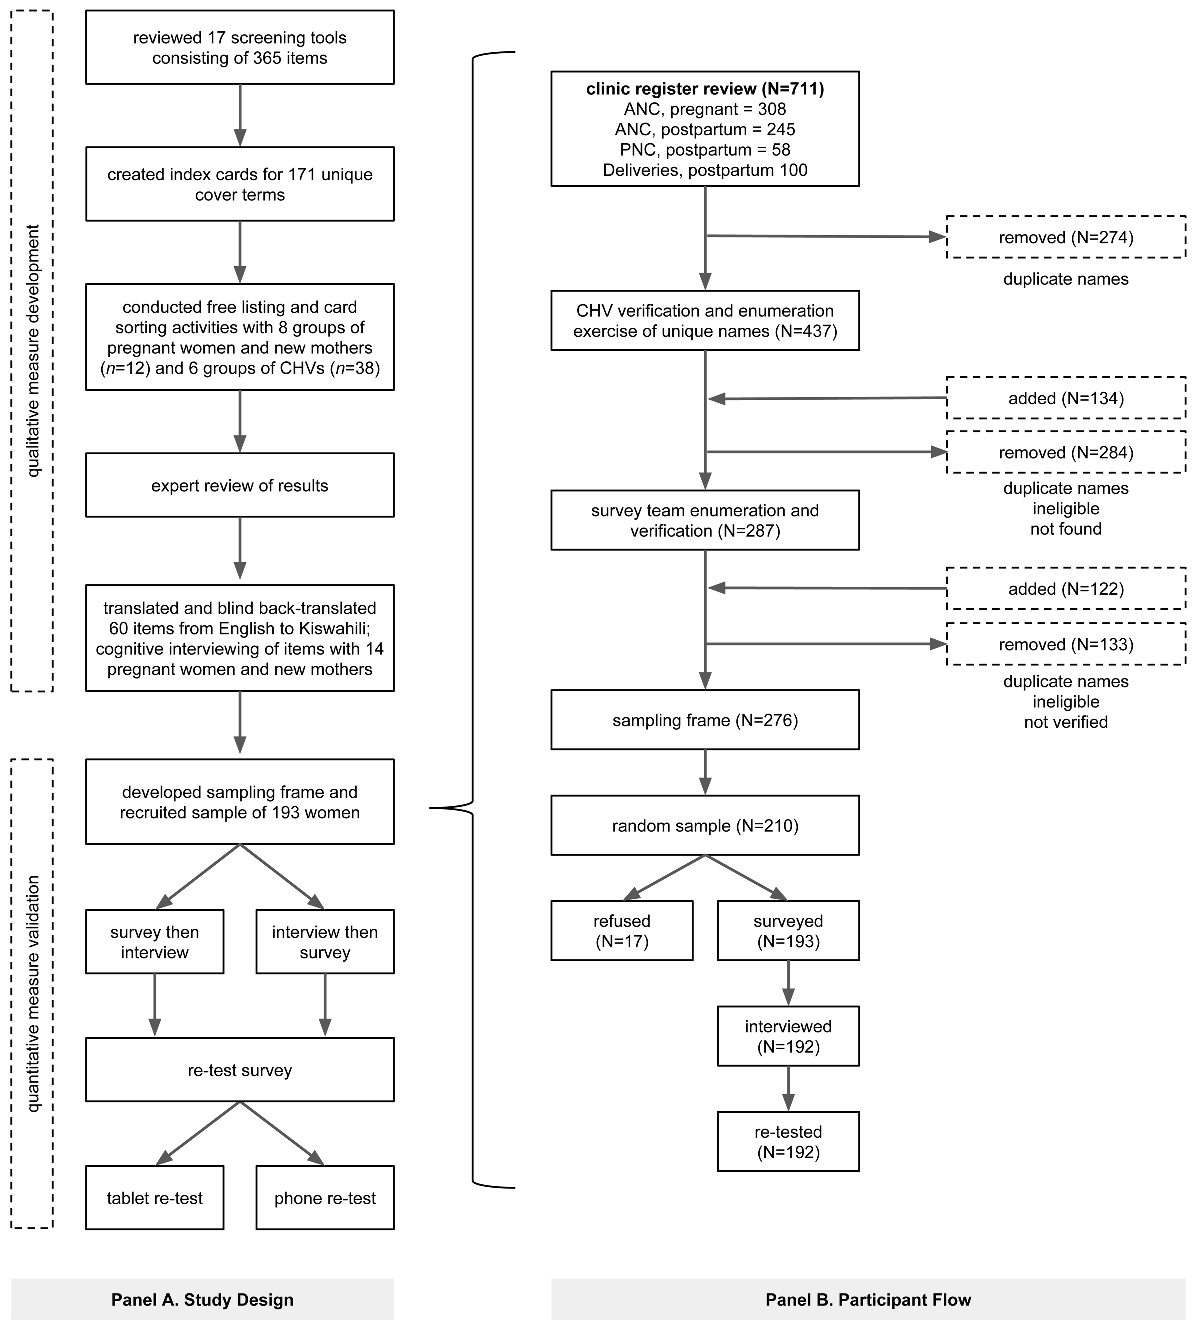
\includegraphics[scale=.8]{figures/designandflow.pdf}
\caption{Panel A: Study design and sequence. Panel B. Participant flow diagram for the diagnostic accuracy study.}
\label{flow}
\end{figure}

\subsubsection{Qualitative Study to Develop Potential Screening Items}

We developed the set of screening items used in the validation study through a process of free listing and card sorting, expert review, and local adaptation. Our objective of this phase of research was to establish the content equivalence, content validity, semantic equivalence, and technical equivalence of the screening items \citep{Kohrt:2011}.

\paragraph{Free listing and card sorting activity (content equivalence)}

Over the course of 7 days in June 2015, we conducted free listing and card sorting exercises with 2 groups of pregnant women and new mothers and 6 groups of CHVs. Free listing is an ethnographic research method that results in a list of responses to a single inquiry \citep{Bolton:2001}. After a brief discussion about the general maternal health issues in the community, we asked each group to list as many characteristics as they could think of in response to a prompt to describe what depression (``sadness'' in Kiswahili) looks like in pregnant women and new mothers. A member of the research team who was fluent in both English and Kiswahili facilitated each discussion and probed for more details throughout the listing procedure. A second researcher took notes and created an index card for each characteristic mentioned by the group.

While the listing exercise was ongoing, a research assistant attempted to match the index cards generated by the group to our set of 171 cover terms (in the client focus groups we only attempted to match against the 54 most common cover terms). After recording direct matches, all non-matching cover term cards were spread out on the table for the group to review. We asked participants to sort the remaining Western psychiatric cards into four piles according to whether the characteristic is something that they observe in the setting: (i) ``yes''; (ii) ``no''; (iii) ``maybe''; or (iv) ``no opinion''. We also tracked how frequently groups generated local constructs (idioms of distress) without matches in the set of Western psychiatric cover terms \citep{Kohrt:2011}. Low literacy levels were not an obstacle as some women in every group were literate.

\paragraph{Expert review (content validity)}

After the completion of the group discussions, a purposive sample of 11 mental health professionals at Moi University Teaching and Referral Hospital was invited by a Kenyan Co-Investigator to review the free listing and card sorting results. Participants included a psychiatrist, two clinical psychologists, and mental health ward nurses. The panel began the session with a discussion of the symptoms identified in the client and CHV free listing exercises, including cultural perceptions of depression and mental health. The expert panel also completed their own free listing activity, similar to the one performed in the client and CHV groups. The researchers attempted to match index cards generated by the panel to the 50 most highly endorsed cover terms from the previous focus groups, and then asked the experts to sort the remaining non-matching cover terms into the same four piles.

\paragraph{Item shortlisting and adaptation (semantic and technical equivalence)}

We created a 60-item screening that we administered to a random sample of pregnant women and new mothers in the validity study. In addition to the 10 EPDS items and the 9 PHQ-9 items, we identified 28 of the most endorsed cover terms and 5 of the most frequently mentioned local constructs. We developed each of these 33 terms into screening items that matched the format and response options of the PHQ-9. For instance, the cover term ``temper'' became ``easily losing your temper'' and followed the format of the PHQ-9 prompt: ``For the past two weeks, how many times have you been bothered by the following problems?'' 

In addition to including the original 10 EPDS items, we also included revised EPDS items that matched the format and response options of the PHQ-9. First, we rephrased the new set of EPDS items so that women could indicate how often they have been bothered by the particular problem in the past two weeks, rather than the past one week (see Table \ref{tbl:epds} in the Online Appendix). Second, we reworded the two `positive' EPDS items to express problems. For example, EPDS item 2 is ``I have looked forward with enjoyment to things.'' In addition to asking women to respond to this original EPDS item, we created a new version phrased as a problem, ``Not looking forward to things''. 

One native speaker translated these 60 items from English to Kiswahili, and a second native speaker conducted the blind back-translation into English. A Kiswahili speaker on the research team resolved discrepancies and conducted cognitive interviewing on the translated items with a convenience sample of 14 pregnant women and new mothers attending the clinic (age \textit{M}=26.0 years, \textit{SD}=4.0 years). The team then adapted the items as necessary to enhance understanding and reviewed the final set with a Kenyan psychiatrist (Co-Investigator).

\subsubsection{Quantitative Study to Validate Measures}

Following the qualitative study, we recruited a probability sample of pregnant women and new mothers to complete three study activities: (i) a 60-item screening consisting of the EPDS, PHQ-9, and our new items; (ii) a re-test within 7 days; and (iii) a semi-structured clinical interview. Our objective of this phase of research was to select the final screening items and to establish the construct validity and diagnostic validity of these items \citep{Kohrt:2011}.

\paragraph{Sampling}

According to the 2014 Kenya DHS, 97.6 percent of women in Bungoma County who gave birth in the previous five years received antenatal care from a skilled provider \citep{KNBS:2015}. So in theory, it should have been sufficient to use the antenatal register as a sampling frame for the population of pregnant women and new mothers living in the catchment area of the clinic. In practice, however, clinic registers can be incomplete and inaccurate. Therefore, working in collaboration with our clinic partner, we created a list of potentially eligible participants based on a review of the antenatal (ANC), postnatal (PNC), and delivery registers before conducting two verification exercises. A detailed participant flow is displayed in Figure \ref{flow}.

We identified 711 study participants who were potentially eligible for a July 2015 study launch: (i) 308 women in the ANC register who were in their second or third trimester, (ii) 245 women in the ANC register who, based on the recorded expected delivery date, should have given birth in the past 1 to 6 months; (iii) 58 women in the PNC register who attended well-baby checkups for babies born in the past 1 to 6 months; and (iv) 100 women in the labor and delivery register who delivered a baby at the facility in the past 1 to 6 months. 437 names remained after de-duplicating the list. 

Next, CHVs for each of the 27 villages within a 2-kilometer radius of the clinic reviewed village-specific lists to verify accuracy and completeness. CHVs added a total of 134 names and removed 284 names of women who were ineligible, not living in the village, or duplicated in the list. The survey team then conducted a second verification exercise on the reduced list of 287 names and further trimmed a net of 11 names, resulting in a sampling frame of 276 women. We drew a simple random sample of 210 women from this sampling frame (see Appendix \ref{app:sample} for a description of the rationale for this sample size). 

\paragraph{Screening and retest}

Three Bachelor's-level Kenyan enumerators with a background in social work or mental health completed one day of training to administer the screening surveys using encrypted Android tablets running ODK Collect (version 1.4.5). Enumerators read the questions aloud and entered the participant's response. Completed data forms were sent daily to a secure research server for processing.

The same enumerator returned within 7 days to complete a re-test survey. Participants were randomized to complete the re-test the same way as before (i.e., the enumerator reading questions on the tablet and entering responses) or via a mobile phone using an automated interactive voice response system. For women who were assigned to the phone re-test, enumerators used a basic mobile phone to call the research number, entered the participant's study information, and then handed the phone to the participant. Women listened privately to automated prompts recorded in Kiswahili and pressed numbers on the phone keypad to respond.

\paragraph{Semi-structured clinical interview}

Women also participated in a semi-structured clinical interview within 3 days of the index test to determine casesness. The order of the survey and interview was randomized at the village level so that roughly half of participants completed the survey before the clinical interview, while the other half completed the interview before the survey. Interviewers and enumerators were blinded to the results and had limited contact with each other during the data collection period. Two Bachelor's-level counselors and two Master's-level counselors were trained by a clinical psychologist (Principal Investigator) and a Kenyan psychiatrist (Co-Investigator) to complete the SCID-5-RV. The team reviewed each section of the interview in detail and then the trainees took turns interviewing a research team member---a native Kiswahili speaker---who played the role of a target woman and followed scripted response sets designed to expose the clinicians to different interview scenarios. In these joint interviews, the non-interviewing trainee also recorded notes and ratings. The pair of clinicians reached 100 percent agreement on the diagnosis across 4 joint interviews.

The Master's-level counselors supervised the research effort and reviewed each completed SCID form and associated clinical notes. During the first week of interviews, the team met in person every evening to review case notes and ratings. Interviewers were trained to report all cases of current suicidal ideation, intent, or attempts, and severe cases of suspected MDE to supervisors for immediate review. With a woman's permission, the interviewer and supervisor made a referral to a counselor in the nearest town or, if necessary, the psychiatric nurse at the district hospital. The research team provided funds to ensure prompt transport and initial care.

\subsection{Analysis}

\subsubsection{Qualitative Study to Develop Potential Screening Items}

We constructed an overall endorsement score for each cover term by averaging the values assigned to each term during the focus group discussions with health workers. If a cover term matched a card generated by a group during the free listing process, the term was assigned a value of `4'. In each group, non-matching cover terms were presented for discussion. Non-matching terms were assigned the following values: `3' if the group endorsed the characteristic, `2' if the group said that the term could be a possible fit, `0' if the group had no opinion, and `-1' if the group rejected the term. We ranked the cover terms by endorsement score and ranked local items without cover term matches by the frequency of mention by the groups. The expert panel reviewed the results with the research team and recommended adding and dropping items from our screening.

\subsubsection{Quantitative Study to Validate Measures}

Our empirical strategy consisted of two phases. First we examined which items did the best job discriminating between cases and non-cases and then assessed which combination of items optimized scale reliability and classification. Second, we assessed the diagnostic validity, construct validity, and reliability of the new scale and two existing scales.

\paragraph{Item analysis}

We adopted an approach to item analysis used in the development of the General Health Questionnaire \citep{Goldberg:1972}. All items had a 4-point response scale ranging from 0 to 3; higher numbers represented more endorsement of the symptom.\footnote{The original 10 EPDS items had a different set of anchors than the other 50 screening items, but the values assigned to each EPDS response option still ranged from 0 to 3, with a value of 3 representing greater problems.} For each item, we calculated the proportion of participants who endorsed the item with a value of 2 or 3. We then subtracted the proportion of endorsement among non-cases from the proportion of endorsement among cases, resulting in a gradient score. 

Items that do a better job discriminating between cases and non-cases have higher gradient scores; negative gradient scores indicate that a higher proportion of non-cases compared to cases endorsed the item. Therefore, we eliminated from further consideration items with a gradient score less than 0.05. We also eliminated items that were endorsed by more than 25 percent of non-cases since non-case endorsement suggests that the item measures a broader, or different construct than depression.
The item analysis resulted in a subset of 20 of the original 60 items that we could further evaluate. 

\paragraph{Item selection}

Using the DSM-5 definition of caseness, we evaluated the internal consistency reliability (Cronbach's alpha) and classification accuracy of all 616,645 possible combinations of these 20 items in scales ranging in size from 2 to 10 items. We used the `OptimalCutpoints' package \citep[version 1.1-3;][]{optimalcutpoints} for R \citep[version 3.2.3;][]{RCoreTeam:2015} to select the optimal cutpoint for each combination of items, giving equal weight to sensitivity and specificity in the identification of cases. We used these results to select the subset of items that would make up the new perinatal depression scale. 

\paragraph{Diagnostic validity}

We report the sensitivity, specificity, accuracy, positive and negative likelihood ratios, and area under the curve for the new perinatal depression scale in addition to the original EPDS and PHQ-9 scales. Confidence intervals for sensitivity and specificity measures are Rubin and Schenker's logit confidence intervals (see L\'{o}pez-Rat\'{o}n et al. \citeyear{optimalcutpoints}). One incomplete observation was dropped.

\paragraph{Construct validity}

To assess convergent validity we calculated the correlation between each measure of depression severity and two measures of functioning: counselor SOFAS rating and client ladder rating. To assess discriminant validity we compared the mean score on each measure of depression severity by caseness.

\paragraph{Reliability}

For the EPDS, PHQ-9, and the new scale, we estimated internal consistency reliability (Cronbach's alpha) for the first test. We also calculated test-retest reliability among the subset of women who completed a tablet re-retest survey within 7 days of the original tablet survey, and among the subset of women who completed a phone re-test survey within the same time period. We tested the null hypothesis of no difference between correlation coefficients by mode of re-test (enumerator administered survey vs automated phone survey) with the `cocor' \citep{Diedenhofen:2015} package that implements Zou's (\citeyear{Zou:2007}) method of calculating confidence intervals on the difference.

\paragraph{Demographics}

We ran cross-tabulations of key demographic variables by maternal status and caseness. In constructing the wealth index from the DHS survey questions we administered, we followed DHS guidance and used reference values from the Kenya 2008-09 DHS \citep{DHSWI}.

\subsection{Research Ethics}

The study protocol was reviewed and approved by the Duke University Institutional Review Board and the Institutional Research and Ethics Committee in Kenya. All team members completed training in research ethics, and all study participants provided written informed consent. A completed STARD checklist is provided in Appendix \ref{app:stard}.

\section{Results}

\subsection{Qualitative Study to Develop Potential Screening Items}

\subsubsection{Participant Characteristics}

We conducted free listing and card sorting exercises with 2 groups of pregnant women and new mothers (\textit{n}=12) and 6 groups of CHVs (\textit{n}=38). On average, groups had 6.2 participants (\textit{SD}=0.9). The average age of the female clients and CHVs was 28.2 (\textit{SD}=3.4) and 41.4 years (\textit{SD}=7.8), respectively. 84.2 percent of CHVs were female, and 55.3 percent finished secondary school. This compared to 33.3 percent of the female clients.

\subsubsection{Item Shortlisting}

The 6 groups of CHVs generated a total of 153 cards (25.5 cards per group; \textit{SD}=3.2).\footnote{As expected, the 2 groups of women generated fewer terms on average compared to the health worker groups (\textit{M}=14.5; \textit{SD}=2.1) and 124 fewer terms overall.} Overall, 58.8 percent of the these cards matched 1 of the 171 Western psychiatric cover terms, supporting the idea that many aspects of depression are universal. We calculated average endorsement scores for each Western cover term and found that the results from CHVs and female clients were highly correlated, \textit{r}(52) = 0.70, \textit{p} <0.001. Since CHVs were asked to discuss the full set of 171 Western psychiatric cover terms, we used their average ratings to select a subset of the most endorsed terms to present to the expert panel, along with several of the most frequently mentioned local idioms of distress not represented in the set of Western terms. The expert panel reviewed and approved of the qualitative results, but added one item for testing: ``feeling like you just want to go back to your maternal home'', a reference to the tradition that women move to the husband's home area upon marriage. In total, we selected 60 items for inclusion in the validation survey.

\subsection{Quantitative Study to Validate Measures}

\subsubsection{Participant Characteristics}

We conducted surveys and interviews with 193 pregnant women and new mothers (clients; 8.1\% refusal). Table \ref{tbl:partSimple} presents participant characteristics by maternal status and compares the study sample to results from the 2014 Kenya DHS \citep{KNBS:2015}. Nearly a third of the sample consisted of pregnant women in their second or third trimester. The sample resembled the broader population of women in terms of literacy, work, parity, and household headship. The women who participated in this study, however, were somewhat poorer and less educated than other women in the region. See Table \ref{tbl:part} in the Online Appendix for additional cross-tabulations by caseness.


\begin{table}[H]
\rotatebox[origin=c]{90}{
\scalebox{1}{
  \centerline{\begin{threeparttable}
  \caption{Participant characteristics by maternal status}
  \label{tbl:partSimple}
  \centering
  \begin{tabular}{lllllll}
  \toprule
  & \multicolumn{3}{c}{Sample} & \multicolumn{2}{c}{Kenya} & \\
  \cmidrule(lr){2-4} \cmidrule(lr){5-6}
  Characteristic & \multicolumn{1}{p{1.5cm}}{\centering Pregnant \\ \textit{n}=61} & \multicolumn{1}{p{1.5cm}}{\centering Postpartum \\ \textit{n}=132} & \multicolumn{1}{p{1.5cm}}{\centering All \\ \textit{n}=193} & Estimate & \multicolumn{1}{c}{Reference} \\
  \midrule
  \expandableinput ../../master/output/tables/part4.tex
  \bottomrule
  \end{tabular}
  \begin{tablenotes}
  \small
  \item 
  \end{tablenotes}
  \end{threeparttable}}}\hspace{3cm}
}
\end{table}

\subsubsection{Prevalence of Depression}

Table \ref{tbl:diagnostic} displays the diagnostic results by maternal status. The overall prevalence of depression ranges from 5.2 to 14.5 percent depending on which reference standard is used. Defining depression based on DSM-5 criteria produces the most conservative estimate of 5.2 percent. In contrast, asking counselors to base their diagnosis of depression on clinical judgment but leaving this unspecified increases the prevalence estimate to 14.5 percent. Requiring concordance between local counselors and clients' assessment of their own functioning produces an estimate of 6.2 percent that is more in line with the DSM-5 estimate. Across all definitions, the prevalence of depression by maternal status reflects the overall prevalence. See Table \ref{tbl:dxpattern} in the Online Appendix to view the pattern of cases and non-cases by case definition.


\begin{table}[H]
%\rotatebox[origin=c]{90}{
\scalebox{1}{
  \centerline{\begin{threeparttable}
  \caption{Diagnostic results by maternal status}
  \label{tbl:diagnostic}
  \centering
  \begin{tabular}{lllll}
  \toprule
  Classifications & \multicolumn{1}{p{1.5cm}}{\centering Pregnant \\ \textit{n}=61} & \multicolumn{1}{p{1.5cm}}{\centering Postpartum \\ \textit{n}=132} & \multicolumn{1}{p{1.5cm}}{\centering All \\ \textit{n}=193} \\
  \midrule
  \expandableinput ../../master/output/tables/part5.tex
  \bottomrule
  \end{tabular}
  \begin{tablenotes}
  \small
  \item 
  \end{tablenotes}
  \end{threeparttable}}%}\hspace{3cm}
}
\end{table}

\subsubsection{Item Analysis}

Figure \ref{gradient} displays the extent to which items discriminated between cases and non-cases. This plot shows each item's gradient score for two different definitions of caseness: DSM-5 (triangle) and counselor clinical judgment (circle). Items with scores to the right of the solid vertical line at zero were endorsed by a higher percentage of cases compared to non-cases. The larger the gradient score, the bigger the difference in endorsement between cases and non-cases. In addition to having large positive gradient scores, items should have low endorsement by non-cases. Items meeting this criterion have a solid black fill. We adopted the 20 items with a gradient score > 0.05 (based on the local definition) and less than 25 percent endorsement by non-cases (solid black shapes to the right of the dashed vertical line). This includes new items such as \texttt{New-19} ``feeling hopeless about the future'' and PHQ-9 items such as \texttt{PHQ-9-3} ``trouble falling or staying asleep, or sleeping too much''.

\begin{figure}[H]
\centering
\includegraphics[scale=.7]{../../master/output/figures/gradient.pdf}
\caption{Item gradients showing discrimination between cases and non-cases, sorted by counselor clinical judgment case definition.}
\label{gradient}
\end{figure}

\subsubsection{Item Selection}

Figure \ref{fig:hexdsm} in the Online Appendix shows a high density scatterplot of the internal consistency reliability and accuracy of all 616,645 combinations of these 20 screening items in sets of 2 through 10. The best combination is a set of 9 items that includes 2 revised EPDS items, 4 items from other Western psychiatric scales, 2 items generated by the focus groups, and 1 item suggested by the expert panel. We refer to this new scale as the Perinatal Depression Screening, or PDEPS. Item psychometrics are presented in Table \ref{tbl:itemstats}. Table \ref{tbl:items} in the Online Appendix lists the English and Kiswahili translations of the PDEPS items.

\begin{table}
\rotatebox[origin=c]{90}{
%\scalebox{.9}{
  \centerline{\begin{threeparttable}
  \caption{PDEPS item statistics}
  \label{tbl:itemstats}
  \centering
  \begin{tabular}{llcccccc}
  \toprule
  & & \multicolumn{2}{c}{DSM-5} & \multicolumn{2}{c}{Local} & & \\
  \cmidrule(lr){3-4} \cmidrule(lr){5-6}
  & & \multicolumn{1}{c}{Non-case} & \multicolumn{1}{c}{Case} & \multicolumn{1}{c}{Non-case} & \multicolumn{1}{c}{Case} & & \multicolumn{1}{c}{Weighted} \\
  Item & Short label & Mean (SD) & Mean (SD) & Mean (SD) & Mean (SD) & Item-Total & \multicolumn{1}{c}{Kappa} \\
  \midrule
  \expandableinput ../../master/output/tables/itemStats.tex
  \bottomrule
  \end{tabular}
  \begin{tablenotes}
  \small
  \item Note. Weighted kappa is reported here as a measure of test-retest reliability at the item-level. Typically the kappa statistic is framed as a measure of inter-rater reliability. For test-retest reliability, an individual woman is the rater at two time points. Since women were responding on an ordinal scale, we calculated weighted kappa to better reflect the degree of agreement or disagreement between time 1 and time 2 (enumerator administration only).
  \end{tablenotes}
  \end{threeparttable}}\hspace{4cm}
}
\end{table}




\subsubsection{Diagnostic Validity}

As shown in Table \ref{tbl:dv}, the optimal cutoff for the new PDEPS tool is greater than or equal to 13. Using this cutoff, the PDEPS correctly classifies 90 percent of clients according to the DSM-5 results, with a sensitivity and specificity of 0.90 and 0.90, respectively. A PDEPS score at or above this cutoff is 8.62 times more likely among women diagnosed with depression than women without a diagnosis (DSM-5). See Table \ref{tbl:dv95} in the Online Appendix for estimates of uncertainty.

The PDEPS outperforms the PHQ-9 and both versions of the EPDS in terms of classification accuracy (DSM-5). The optimal cutoff scores for the original EPDS and PHQ-9 are 16 and 15, respectively---higher than what most of the published literature would recommend (see \citep{kroenke:2001} and Table \ref{tbl:epdscompare} in the Online Appendix). While the estimates of sensitivity and specificity are lower for the EPDS and PHQ-9 compared to the PDEPS, these estimates are within the range of what is reported in the literature. Table \ref{tbl:epdscompare} compares these results to other studies of the EPDS in African countries.

The PDEPS also outperforms the EPDS and PHQ-9 in classifying depression according to the `local' definition---concordance between counselor clinical judgment and client rating of functioning---but the evidence is more equivocal. The PDEPS correctly classifies more true negatives and is more accurate overall compared to the other scales, but it has a higher false negative rate. 


\begin{table}
\rotatebox[origin=c]{90}{
%\scalebox{.9}{
  \centerline{\begin{threeparttable}
  \caption{Diagnostic validity}
  \label{tbl:dv}
  \centering
  \begin{tabular}{llllllllllllll}
  \toprule
  & & \multicolumn{6}{c}{DSM-5} & \multicolumn{6}{c}{Local} \\
  \cmidrule(lr){3-8} \cmidrule(lr){9-14}
  Scale & Cut & Sen & Spe & Acc & LRP & LRN & AUC & Sen & Spe & Acc & LRP & LRN & AUC \\
  \midrule
  \textit{Combined, N=193} & & & & & & & & & & & & & \\
  \expandableinput ../../master/output/tables/dv.tex
  \midrule
  \textit{Pregnant, n=61} & & & & & & & & & & & & & \\
  \expandableinput ../../master/output/tables/dvPr.tex
  \midrule
  \textit{Postpartum, n=132} & & & & & & & & & & & & & \\
  \expandableinput ../../master/output/tables/dvPp.tex
  \bottomrule
  \end{tabular}
  \begin{tablenotes}
  \small
  \item Note. Sen=sensitivity. Spe=specificity. Acc=accuracy (1-error rate). LRP=likelihood ratio (positive). LRN=likelihood radio (negative). AUC=area under the receiver operating characteristic curve.
  \end{tablenotes}
  \end{threeparttable}}\hspace{4cm}
}
\end{table}



\subsubsection{Construct Validity}

All scales discriminate between cases and non-cases. As shown in Table \ref{tbl:cv}, the mean PDEPS score among cases is twice as large as the mean score among non-cases. The difference between cases and non-cases is smaller for the other scales, but still statistically significant. Each scale is also negatively correlated with the client and counselor ratings of client functioning, exhibiting the expected inverse relationship between depression severity and functioning. The magnitude of these correlations ranges from -0.24 to -0.38, providing evidence of convergent validity.

\begin{table}
\rotatebox[origin=c]{90}{
%\scalebox{.9}{
  \centerline{\begin{threeparttable}
  \caption{Construct validity}
  \label{tbl:cv}
  \centering
  \begin{tabular}{llllllllll}
  \toprule
  & & \multicolumn{6}{c}{Discriminant Validity} & \multicolumn{2}{c}{Convergent Validity} \\
  \cmidrule(lr){3-8} \cmidrule(lr){9-10}
  & \multicolumn{1}{c}{All} & \multicolumn{3}{c}{DSM-5} & \multicolumn{3}{c}{Local} & \multicolumn{2}{c}{\textit{r} functioning} \\
  \cmidrule(lr){2-2} \cmidrule(lr){3-5} \cmidrule(lr){6-8} \cmidrule(lr){9-10}
   & & \multicolumn{1}{c}{Non-case} & \multicolumn{1}{c}{Case} & & \multicolumn{1}{c}{Non-case} & \multicolumn{1}{c}{Case} & & \multicolumn{1}{c}{Client} & \multicolumn{1}{c}{Counselor} \\
  Scale & \multicolumn{1}{c}{Mean (SD)} & \multicolumn{1}{c}{Mean (SD)} & \multicolumn{1}{c}{Mean (SD)} & \multicolumn{1}{c}{Diff (\%)} & \multicolumn{1}{c}{Mean (SD)} & \multicolumn{1}{c}{Mean (SD)} & \multicolumn{1}{c}{Diff (\%)} & \multicolumn{1}{c}{Rating} & \multicolumn{1}{c}{Rating} \\
  \midrule
  \expandableinput ../../master/output/tables/conv.tex
  \bottomrule
  \end{tabular}
  \begin{tablenotes}
  \small
  \item Note. * \textit{p}<0.05. ** \textit{p}<0.01. *** \textit{p}<0.001.
  \end{tablenotes}
  \end{threeparttable}}\hspace{4cm}
}
\end{table}




\subsubsection{Reliability}

Table \ref{tbl:rel} presents estimates of internal consistency and test-retest reliability. Each scale demonstrates acceptable internal consistency reliability as measured by Cronbach's alpha, ranging from 0.77 to 0.83. Estimates of test-retest reliability range from 0.57 to 0.67 across scales for identical administration within 7 days (see Table \ref{tbl:itemstats} for estimates of item-level test-retest reliability). Estimates are smaller for retests administered via an automated phone service---from 0.36 to 0.53---but the difference was not statistically significant in all cases.

If women perceived automated phone administration to be more private and confidential, phone retests would be expected to be less reliable as women report more symptoms of depression over the phone. To test this hypothesis, we regressed depression scores on an indicator of phone retest. As shown in Table \ref{tbl:phone} in the Online Appendix, mean depression scores are up to 19.9 percent higher among women who were randomly assigned to complete the retest via the automated phone service compared to women who responded to questions read by an enumerator.

\begin{table}
\rotatebox[origin=c]{90}{
%\scalebox{.9}{
  \centerline{\begin{threeparttable}
  \caption{Internal consistency and test-retest reliability}
  \label{tbl:rel}
  \centering
  \begin{tabular}{llllllllll}
  \toprule
  & \multicolumn{2}{c}{Internal Consistency} & \multicolumn{7}{c}{Test-retest} \\
  \cmidrule(lr){2-3} \cmidrule(lr){4-10}
  & & & \multicolumn{2}{c}{Enumerator} & \multicolumn{2}{c}{Automated phone} & \multicolumn{3}{c}{Difference} \\
  \cmidrule(lr){4-5} \cmidrule(lr){6-7} \cmidrule(lr){8-10}
  Scale & \textit{N} & Alpha & \textit{n} & \textit{r} & \textit{n} & \textit{r} & \textit{r} & L95\% & U95\% \\
  \midrule
  \expandableinput ../../master/output/tables/rel.tex
  \bottomrule
  \end{tabular}
  \begin{tablenotes}
  \small
  \item Note. Women were randomized to complete a re-test survey with the same enumerator who read the questions and recorded responses (same method as the first administration) or via an automated phone screening.
  \end{tablenotes}
  \end{threeparttable}}\hspace{4cm}
}
\end{table}




\subsubsection{Correlates of Depression}

Table \ref{tbl:det} reports the correlates of the PDEPS score. There is an inverse relationship between household wealth and depression such that women from wealthier households endorsed fewer symptoms of depression. At the same time, however, work is associated with more depression. Living with a spouse or partner is also associated with lower depression scores, but this relationship is not statistically significant.  

\input{../../master/output/tables/det.tex}

\section{Discussion}

This study demonstrates that the EPDS and PHQ-9 screening tools have acceptable sensitivity and specificity for detecting major depressive episode (DSM-5) among pregnant women and new mothers in Kenya. The EPDS diagnostic validity results are at the low end of what is reported in other studies of African samples, and our recommended cutoff of $\geq$ 16 is notably higher that what these other studies report (see Tsai et al. \citeyear{Tsai:2013} and Table \ref{tbl:epdscompare} in the Online Appendix), but our results confirm that the EPDS and PHQ-9 are valid instruments for this setting. They may not be not optimal, however.

The new scale we developed through a process of free listing, card sorting, and item analysis---the Perinatal Depression Screening, or PDEPS---performs better on all metrics of classification accuracy with respect to DSM-5 caseness. We recruited too few pregnant women to make strong conclusions about the diagnostic validity of the PDEPS with respect to detecting depression during the antenatal period, but overall classification accuracy was high. Our postpartum sample was twice as large, however, and results suggest that the PDEPS outperforms the EPDS and PHQ-9 in terms of diagnostic accuracy during this period.

We developed the PDEPS through a hybrid emic and etic approach that blended Western psychiatric concepts with locally derived idioms of distress. This work drew inspiration from several previous studies that took a similar approach to combining Western and indigenous concepts \citep[e.g.,][]{Bass:2008,Kaaya:2008,Nhiwatiwa:1998,Patel:1997}. In particular, we can compare our results to Bass et al. (\citeyear{Bass:2008}) who used similar methods in the Democratic Republic of Congo to develop and validate a locally-derived measure of postpartum depression (\textit{Maladi ya Souci}, a syndrome of worry) that contained some EPDS items. The authors found that their 16-item local syndrome scale performed similarly to a shorter version of the EPDS and another Western scale in terms of diagnostic accuracy.

Unlike Bass et al. (\citeyear{Bass:2008}) who found that their locally-derived scale included all of the diagnostic symptom categories for MDD, we found that the best combination of items on the PDEPS deviates somewhat from DSM-5 criteria. For instance, one of the most discriminating items, ``Feeling like you just want to go back to your maternal home'', was suggested by the expert panel of Kenyan mental health professionals who are trained from a Western model but whose practice is informed by local customs. This particular custom refers to the tradition that women often leave their maternal home upon marriage and resettle in their husband's village. Wanting to go back to your maternal home would signal difficulty coping with present circumstances. Given the culturally-anchored nature of this item, some adaptation might be required if the PDEPS is to be used in other settings where this behavior is not a custom. Other PDEPS items more clearly reflect the universal nature of depression, such as ``feeling hopeless'', ``feeling anxious or worried for no good reason'', and ``crying because of sadness''---the latter two overlapping directly with the EPDS.

The study by Bass et al. (\citeyear{Bass:2008}) is also an interesting comparison because the authors did not rely on standard clinical interviews to assess caseness. Instead, they considered a woman a `case' if a key informant identified her as suffering from the local syndrome \textit{and} if the woman self-identified as having the syndrome. In addition to using the SCID-5-RV as a reference criterion, we also separately examined `local' cases defined by concordance between a counselor's clinical judgment---not bound by DSM-5 criteria---and the woman's self-report of poor functioning. As far as we know, ours is the first study to compare Western and local approaches to define caseness.

Interestingly, both definitions of caseness lead to a similar overall estimate of prevalence: 5.2 percent using a DSM-5 gold-standard interview and 6.2 percent using a local definition based on concordance between counselor clinical judgment and client self-assessment. These results are internally consistent, but represent a divergence from other published prevalence estimates. For instance, a systematic review by Villegas et al. (\citeyear{Villegas:2011}) reported a point estimate of 31.3 percent in developing countries (95\%CI 21.3 to 43.5). Another systematic review of common perinatal mental disorders in low- and lower-middle-income countries---so a broader scope than just depressive disorders---estimated an overall prevalence of 18.6 percent \citep[95\%CI 18.0 to 19.2;][]{Fisher:2012}. A third systematic review limited to studies of African samples---but none conducted in Kenya---reported a prevalence of depression of 11.3 percent during the antenatal period (95\%CI 9.5 to 13.1) and 18.3 percent during the postnatal period \citep[95\%CI 17.5 to 19.1;][]{Sawyer:2010}.

If we relax the requirement for concordance and consider only counselor clinical judgment, our estimate of prevalence increases to 14.5 percent. This might be most comparable to the Fisher et al. (\citeyear{Fisher:2012}) estimate of 18.6 percent for common perinatal mental disorders, assuming that counselors in our study might have considered a broader range of symptoms than strictly depression when labeling cases when relying on their clinical judgment. In any case, this higher estimate should probably be considered an upper-bound on prevalence with an understanding that the DSM-5 gold-standard and the local concordance gold-standard produces estimates half as large.

While this study affirms the validity of screening for perinatal depression, it also raises an interesting question about how to implement screening at scale. Low literacy rates in places like rural Kenya preclude a complete reliance on self-administration. Nurse-administered screenings are of course possible at primary health centers, but this approach is limited by other demands on staff time and the need for additional training. These are barriers that can be overcome, however there is still the issue that facility-based screening will not reach all pregnant women and new mothers, particularly in settings were antenatal care is not universal and where rates of facility delivery remain low. To increase coverage, we should consider how automated screenings delivered via phone calls could help to overcome all of these barriers.

We examined the test-retest reliability of automated phone administration and found that retest surveys conducted via interactive voice response were somewhat less reliable than in-person retest surveys administered by the same enumerator. However, we hypothesized that the private nature of automated phone administration would lead to more endorsement of depression symptoms, thus making the phone retests appear less reliable. This is what we found, and it is consistent with other research on interactive voice response systems. Kobak et al. (\citeyear{Kobak:1999}) found that U.S. patients reported more embarrassment in acknowledging depression symptoms to a live clinician compared to an automated voice system, and Lieberman et al. (\citeyear{ Lieberman:2012}) reviewed the use of automated voice screening for medical research and concluded that automated interviews give patients a sense of anonymity that leads to increased reporting compared to in-person interviews. More work is needed to understand the potential uses of and barriers to automated screening at scale in low-income countries, particularly for rural health systems.

Phone screenings would also offer the opportunity to assess voice samples. All of the current methods of screening for depression, assessing severity, and monitoring response to treatment rely on either patient-report or clinician judgment, both of which can be subjective and error prone. The search for more objective biomarkers of depression has led researchers to study how depression affects speech. Findings from a recent randomized controlled trial in the U.S. demonstrated that it is feasible to obtain valid measures of depression severity and response to treatment via the analysis of vocal recordings captured via an automated phone system \citep{Mundt:2012}. As part of a Phase 4 randomized trial of treatments for Major Depression, 105 patients assigned to treatment arms provided speech samples in addition to completing several clinical assessments of depression severity and response to treatment. The study found that changes in speech patterns were associated with clinical outcomes, suggesting that there may be clinically important vocal biomarkers of depression. This represents a potentially important new direction for research in wide-scale depression screening in low-income settings.

\subsection{Limitations}

A strength of the current study was the development of a community sampling frame and the use of probability sampling. As demonstrated in the results, the sample of pregnant women and new mothers recruited for this study resembled women in the region in many respects. Despite being representative, however, our sample was recruited from a relatively small catchment area---a 2 kilometer radius around a particular primary health center. The results may generalize to other rural areas in the region, but it is not clear how the findings might apply in different regions or urban areas. Also, while this study addressed the antenatal and postnatal period, the sample size was not large enough to permit a full investigation of differences by period. A lower than expected prevalence rate led to wide confidence intervals on estimates of sensitivity given the sample size. Additionally, it is important to note that the gold-standard SCID-5-RV itself has not been specifically validated in Kenya as far as we know, but the DSM-5 on which it is based is the diagnostic standard for mental health professionals in Kenya. It is also worth noting that participants did not complete the survey and clinical interviews on the same day, but the order of completion was balanced by random assignment. 

\subsection{Conclusions}

The EPDS and PHQ-9 are valid and reliable screening tools for perinatal depression in rural Western Kenya, but a new 9-item locally-developed tool called the Perinatal Depression Screening (PDEPS) that blends Western psychiatric concepts and local idioms of distress may be a more useful alternative. At less than 10 percent, the prevalence of depression in this region appears to be lower than other published estimates for African and other low-income countries. Additional research is needed to confirm this finding and to explore how to implement depression screening at scale, potentially through mobile phones and automated voice services. Additional research is also needed to develop and validate instruments for co-morbid symptoms of anxiety during the perinatal period.


%------------------------------------------------------------------------------
\bibliographystyle{apacite}
\bibliography{../peridep}

\processdelayedfloats

\makeatletter
\efloat@restorefloats
\makeatother
\setcounter{figure}{0} % Start again
\renewcommand\thefigure{A.\arabic{figure}}
\setcounter{table}{0} % Start again
\renewcommand\thetable{A.\arabic{table}}

\clearpage
\pagenumbering{roman}

\appendix
\section{Supplemental Tables and Figures}
\label{app:stf}

\newpage
\begin{table}
%\scalebox{.9}{
  \centerline{\begin{threeparttable}
  \caption{Measures of depression reviewed}
  \label{tbl:measures}
  \centering
  \begin{tabular}{ll}
  \toprule
  Measures & Items \\
  \midrule
  \expandableinput ../../master/output/tables/measures.tex
  \bottomrule
  \end{tabular}
  \begin{tablenotes}
  \small
  \item Note. We removed items included in the ``Core'' and ``Standard'' versions of the Pregnancy Risk Assessment Monitoring System (PRAMS) and the Bromley Postnatal Depression Scale (BPDS) because the scales assess a patient's history rather than her depressive symptoms. For instance, the BPDS includes items such as ``Did you talk to a psychiatrist because you felt depressed during the first year after the baby was born?'' An example PRAMS ``Core'' item is ``Thinking back just before you got pregnant with your new baby, how did you feel about becoming pregnant?''.
  \end{tablenotes}
  \end{threeparttable}}%}
\end{table}




\newpage
\begin{table}
%\rotatebox[origin=c]{90}{
%\scalebox{0.9}{
  \centerline{\begin{threeparttable}
  \caption{Modifications to the SCID-5-RV}
  \label{tbl:scid}
  \centering
  \begin{tabular}{p{1in}p{5in}}
  \toprule
  Module & Modification \\
  \midrule
  overview & The sections on demographic data and alcohol and drug use were reduced. \\
  overview & Added: ``Imagine a ladder with 10 steps. On the bottom step, Step 1, are women who are really struggling and not doing well. On the top step, Step 10, are women who are doing very well. On which step do you stand?'' \\
  A & The following MDE specifiers were not included: with mixed features, with catatonia, with melancholic features, and with atypical features \\
  A & Past MDE not assessed \\
  A & Other mood disorders not assessed \\
  A & Raters could not rule out depression due to another medical condition or a substance; rather they were prompted to investigate and flag the case for discussion \\
  D & Other mood disorders not assessed \\
  D & For MDD, Criterion E not assessed \\
  D & MDD type not assessed \\
  D & MDD seasonal pattern not assessed \\
  D & MDD congruency of psychotic symptoms not assessed \\
  D & MDD with panic attacks not assessed \\
  D & Raters could not rule out depression due to another medical condition or a substance; rather they were prompted to investigate and flag the case for discussion \\
  \bottomrule
  \end{tabular}
  \begin{tablenotes}
  \small
  \item Note. MDE = Major Depressive Episode. MDD = Major Depressive Disorder.
  \end{tablenotes}
  \end{threeparttable}}%}\hspace{4cm}
%}
\end{table}


\newpage
\begin{table}
\rotatebox[origin=c]{90}{
%\scalebox{.9}{
  \centerline{\begin{threeparttable}
  \caption{EPDS revisions}
  \label{tbl:epds}
  \centering
  \begin{tabular}{lll}
  \toprule
  Item & Original & Revised \\
  \midrule
  1 & I have been able to laugh and see the funny side of things & ...feeling unable to laugh or have fun \\
  2 & I have looked forward with enjoyment to things & ...not looking forward to things \\
  3 & I have blamed myself unnecessarily when things went wrong & ...blaming yourself when things go wrong \\
  4 & I have been anxious or worried for no good reason & ...feeling anxious or worried for no good reason \\
  5 & I have felt scared or panicky for no very good reason & ...feeling scared or panicky for no good reason \\
  6 & Things have been getting on top of me & ...feeling overwhelmed \\
  7 & I have been so unhappy that I have had difficulty sleeping & ...trouble sleeping at night \\
  8 & I have felt sad or miserable & ...feeling sad or miserable \\
  9 & I have been so unhappy that I have been crying & ...crying because of sadness \\
  10 & Thoughts of harming myself have occurred to me & ...thoughts of harming yourself \\
  \bottomrule
  \end{tabular}
  \begin{tablenotes}
  \small
  \item Note. In addition to including the original 10 EPDS items, we also included revised EPDS items that matched the format and response options of the PHQ-9. First, we rephrased the new set of EPDS items so that women could indicate how often they have been bothered by the particular problem in the past two weeks, rather than the past one week. Second, we reworded the three `positive' EPDS items to express problems.
  \end{tablenotes}
  \end{threeparttable}}\hspace{3cm}
}
\end{table}




\newpage
\begin{table}
\scalebox{.75}{
  \begin{threeparttable}
  \caption{Participant characteristics by maternal status and caseness}
  \label{tbl:part}
  %\centering
  \begin{tabular}{lllllllll}
  \toprule
  & \multicolumn{3}{c}{Non-cases} & \multicolumn{3}{c}{Cases} & \\
  \cmidrule(lr){2-4} \cmidrule(lr){5-7}
  Case Definition/Characteristic & Pregnant & Postpartum & Both & Pregnant & Postpartum & Both & All \\
  \midrule
  \textit{DSM-5 Diagnosis$\dagger$} & & & & & & & \\
  \expandableinput ../../master/output/tables/part.tex
  \midrule
  \textit{Local, Counselor-Client Concordance} & & & & & & & \\
  \expandableinput ../../master/output/tables/part2.tex
  \midrule
  \textit{Local, Counselor Only} & & & & & & & \\
  \expandableinput ../../master/output/tables/part3.tex
  \bottomrule
  \end{tabular}
  \begin{tablenotes}
  \small
  \item Note. $\dagger$ Major Depressive Episode or Other specified depressive disorder.
  \end{tablenotes}
  \end{threeparttable}
}
\end{table}


\newpage
\begin{table}
%\rotatebox[origin=c]{90}{
%\scalebox{.9}{
  \centerline{\begin{threeparttable}
  \caption{Pattern of diagnostic results}
  \label{tbl:dxpattern}
  \centering
  \begin{tabular}{llll}
  \toprule
  Definition & Count & \% & Cumlative \% \\
  \midrule
  \expandableinput ../../master/output/tables/dxtbl.tex
  \bottomrule
  \end{tabular}
  \begin{tablenotes}
  \small
  \item 
  \end{tablenotes}
  \end{threeparttable}}%}
%}
\end{table}




\newpage
\begin{table}
%\rotatebox[origin=c]{90}{
%\scalebox{.9}{
  \centerline{\begin{threeparttable}
  \caption{Perinatal Depression Screening (PDEPS)}
  \label{tbl:items}
  \centering
  \begin{tabular}{llp{2in}p{2in}}
  \toprule
  Item & Source & English & Kiswahili \\
  \midrule
  \expandableinput ../../master/output/tables/itemWording.tex
  \bottomrule
  \end{tabular}
  \begin{tablenotes}
  \small
  \item Note. ``Western'' indicates that the item came from an existing screening tool. ``Local'' indicates that the item was generated by one or more of the focus group discussions.
  \end{tablenotes}
  \end{threeparttable}%}\hspace{4cm}
}
\end{table}




%\newpage

\begin{table}
\rotatebox[origin=c]{90}{
%\scalebox{.9}{
  \centerline{\begin{threeparttable}
  \caption{Uncertainty in diagnostic validity}
  \label{tbl:dv95}
  \centering
  \begin{tabular}{llllllllllllll}
  \toprule
  & & \multicolumn{6}{c}{DSM-5} & \multicolumn{6}{c}{Local} \\
  \cmidrule(lr){3-8} \cmidrule(lr){9-14}
  & & \multicolumn{3}{c}{Sensitivity} & \multicolumn{3}{c}{Specificity} & \multicolumn{3}{c}{Sensitivity} & \multicolumn{3}{c}{Specificity} \\
  \cmidrule(lr){3-5} \cmidrule(lr){6-8} \cmidrule(lr){9-11} \cmidrule(lr){12-14}
  Scale & Cut & Est & L95 & U95 & Est & L95 & U95 & Est & L95 & U95 & Est & L95 & U95 \\
  \midrule
  \textit{Combined, N=193} & & & & & & & & & & & & & \\
  \expandableinput ../../master/output/tables/dv95.tex
  \midrule
  \textit{Pregnant, n=61} & & & & & & & & & & & & & \\
  \expandableinput ../../master/output/tables/dv95Pr.tex
  \midrule
  \textit{Postpartum, n=132} & & & & & & & & & & & & & \\
  \expandableinput ../../master/output/tables/dv95Pp.tex
  \bottomrule
  \end{tabular}
  \begin{tablenotes}
  \small
  \item Note. 95 percent confidence intervals reported.
  \end{tablenotes}
  \end{threeparttable}}\hspace{4cm}
}
\end{table}

%\newpage

\begin{table}
\rotatebox[origin=c]{90}{
\scalebox{.80}{
  \centerline{\begin{threeparttable}
  \caption{Comparison of EPDS diagnostic validity results across African samples}
  \label{tbl:epdscompare}
  \centering
  \begin{tabular}{lllllllllll}
  \toprule
  Study & Country & Sample & Criterion & Period & Case-Control & Uniform & Blinding & Cutoff & Sen & Spe \\
  \midrule
  CURRENT STUDY & Kenya & Community & SCID-5-RV & Antenatal/postnatal (4-36 wk) & No & Yes & Yes & $\geq$ 16 & 0.70 & 0.72 \\
  \midrule
  \expandableinput ../../master/output/tables/epdscompare.tex
  \bottomrule
  \end{tabular}
  \begin{tablenotes}
  \small
  \item Note. Table reproduced in part from Tsai et al. (\citeyear{Tsai:2013}). CPRS = Comprehensive Psychopathological Rating Scale. MINI = Mini International Neuropsychiatric Interview. PSE = Present State Examination. SADS = Schedule for Affective Disorders and Schizophrenia. SCID = Structured Clinical Interview for the Diagnostic and Statistical Manual of Mental Disorders. Case-control study design: reference criterion is established in a subset of participants based on the results of the index test. Non-uniform test: index test is not administered in a uniform fashion. Blinded: reference criterion is administered and/or assessed without knowledge of the index test results. Sen = Sensitivity. Spe = Specificity. Weobong et al. (\citeyear{Weobong:2009}) also assessed the diagnostic validity of the PHQ-9 among new mothers in Ghana and found that a cutoff of $\geq$ 5 had a sensitivity and specificity of 0.94 and 0.75, respectively.
  \end{tablenotes}
  \end{threeparttable}}\hspace{2cm}
}}
\end{table}

\newpage
\begin{table}
%\rotatebox[origin=c]{90}{
%\scalebox{.9}{
  \centerline{\begin{threeparttable}
  \caption{Regression of depression severity score on indicator of automated phone administration}
  \label{tbl:phone}
  \centering
  \begin{tabular}{lllllll}
  \toprule
  & \multicolumn{1}{c}{Enumerator} & \multicolumn{5}{c}{Automated phone} \\
  \cmidrule(lr){2-2} \cmidrule(lr){3-7}
  Scale & Mean & Est & StdErr & \% Diff & \textit{t} & \textit{p} \\
  \midrule
  \expandableinput ../../master/output/tables/phone.tex
  \bottomrule
  \end{tabular}
  \begin{tablenotes}
  \small
  \item Note. Women were randomized to complete a re-test survey with the same enumerator who read the questions and recorded responses (same method as the first administration) or via an automated phone screening.
  \end{tablenotes}
  \end{threeparttable}%}\hspace{4cm}
}
\end{table}




\begin{figure}
\centering
\includegraphics[scale=.8]{../../master/output/figures/aucValpha_DSM.pdf} %
\caption{High density scatterplot of the internal consistency reliability and accuracy of all 616,645 combinations of 20 screening items in sets of 2 through 10. DSM-5 definition of depression.}
\label{fig:hexdsm}
\end{figure}

\newpage
\section{Rationale for Sample Size}
\label{app:sample}
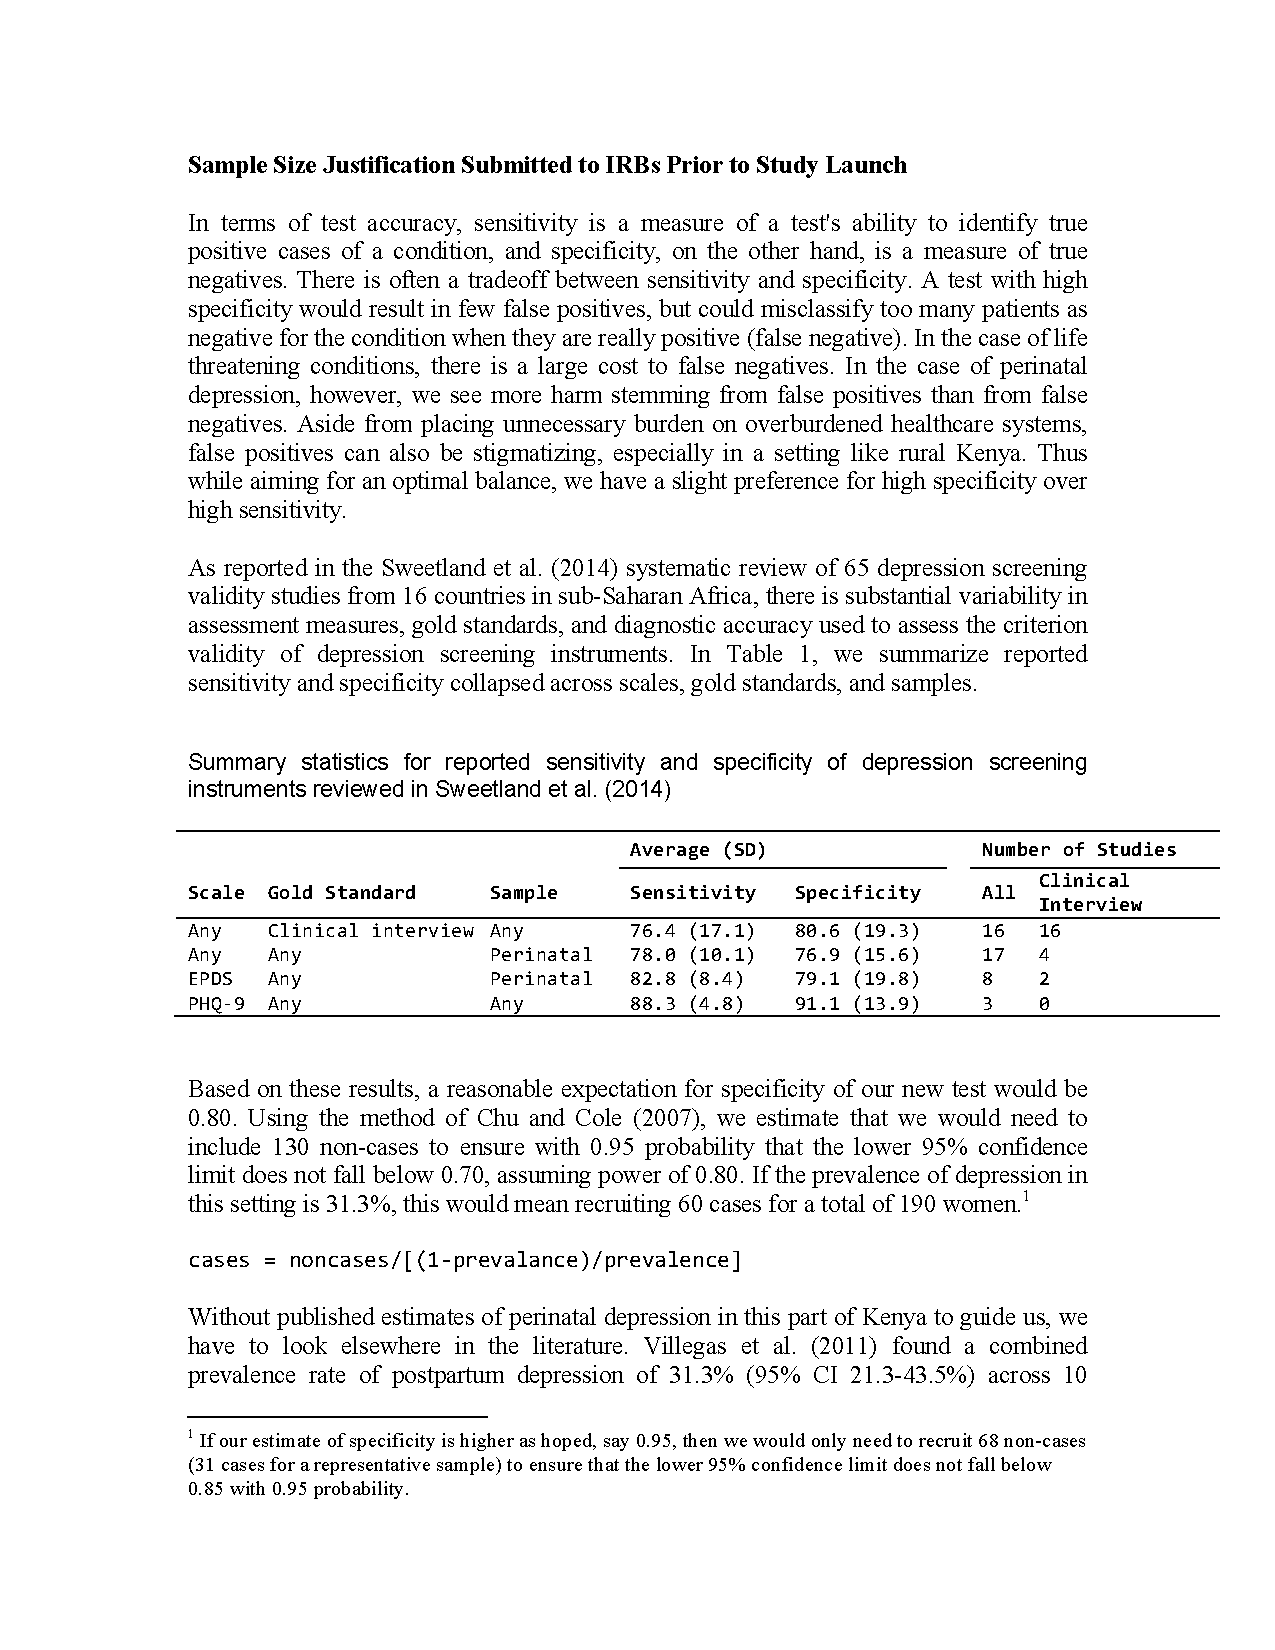
\includepdf[pages=-,]{supplemental/sample.pdf}

\newpage
\section{STARD Checklist}
\label{app:stard}
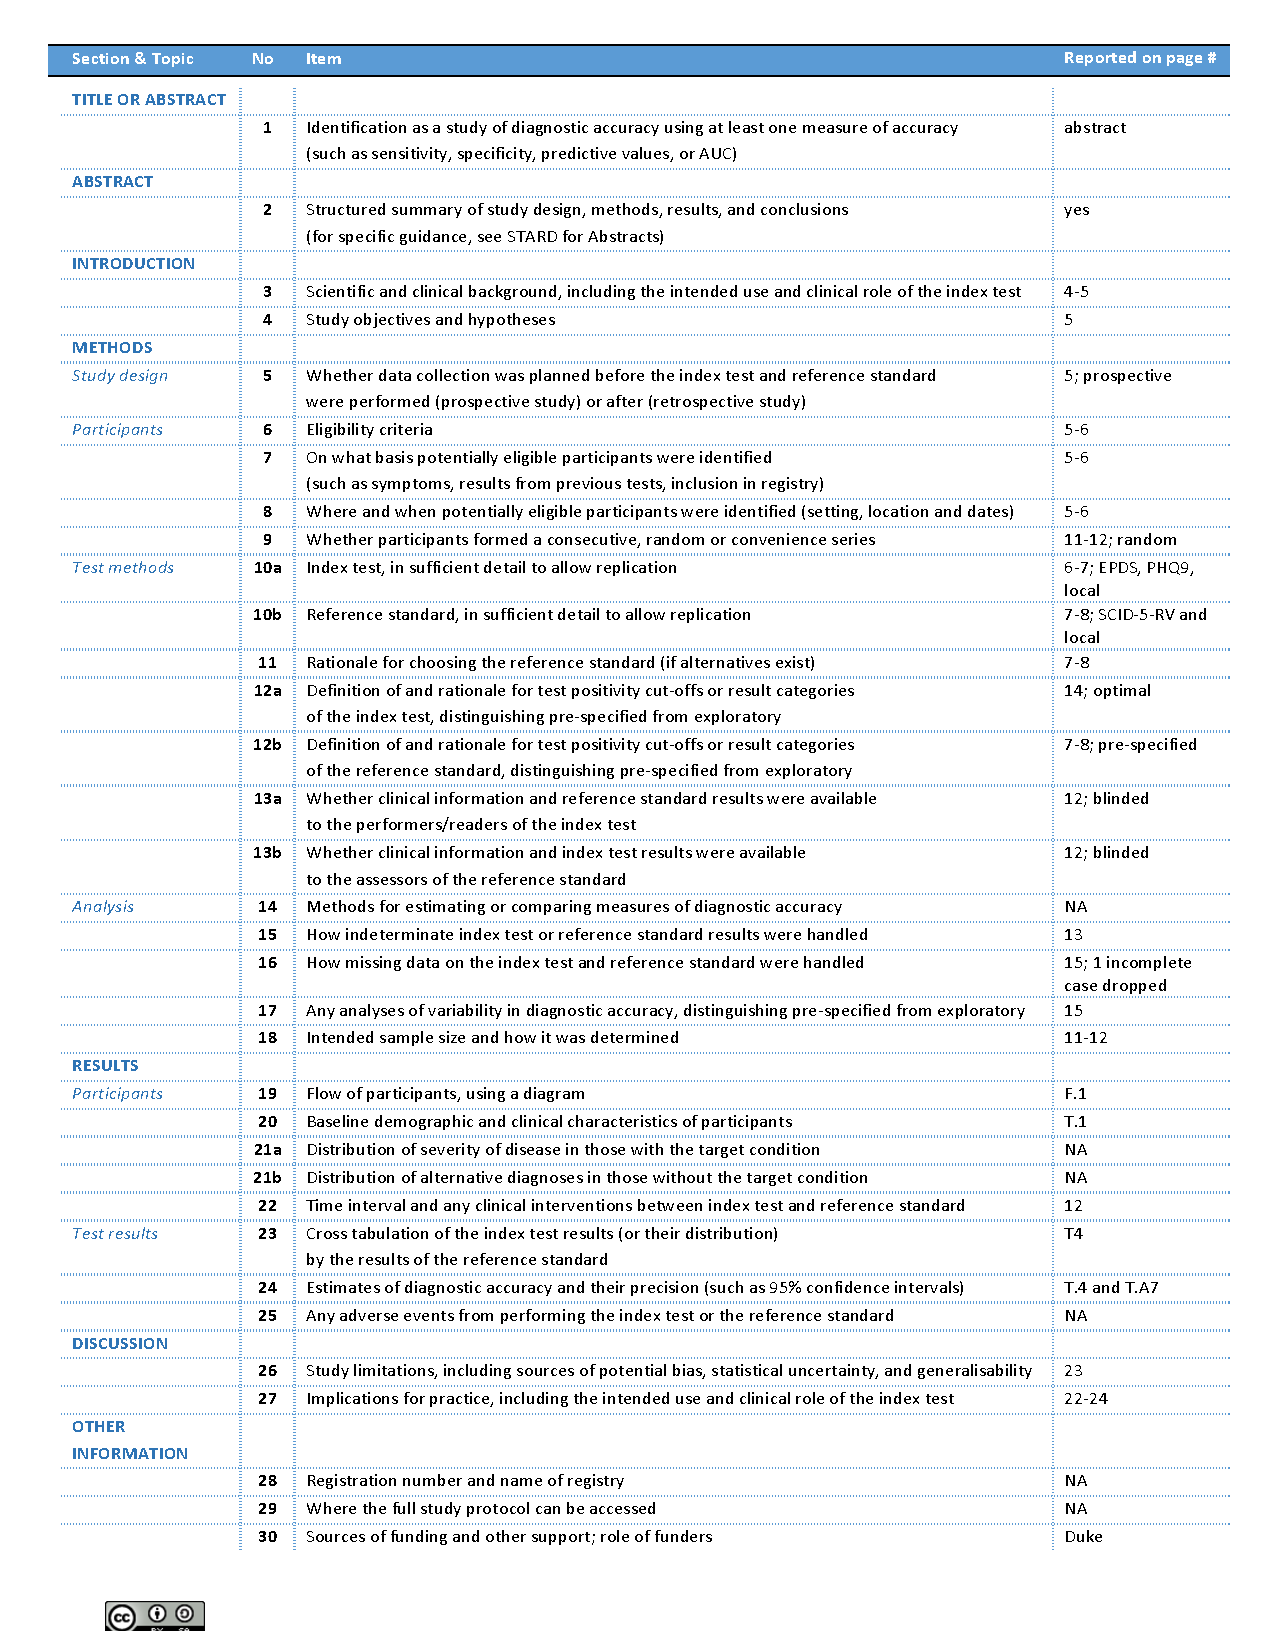
\includepdf[pages=-,]{supplemental/stard.pdf}

\newpage

{\parindent0pt

\textbf{References}

Abiodun, O. A. (2006). Postnatal depression in primary care populations in Nigeria. \textit{General Hospital Psychiatry, 28(2)}, 133--136.

\vspace{0.25cm}

Adewuya, A. O. (2006). Early postpartum mood as a risk factor for postnatal depression in Nigerian women. \textit{The American Journal of Psychiatry, 163(8)}, 1435--1437.

\vspace{0.25cm}

Adewuya, A. O., Eegunranti, A. B., \& Lawal, A. M. (2005). Prevalence of postnatal depression in Western Nigerian women: a controlled study. \textit{International Journal of Psychiatry in Clinical Practice, 9(1)}, 60--64.

\vspace{0.25cm}

Adewuya, A. O., Ola, B. A., Dada, A. O., \& Fasoto, O. O. (2006). Validation of the Edinburgh Postnatal Depression Scale as a screening tool for depression in late pregnancy among Nigerian women. \textit{Journal of Psychosomatic Obstetrics and Gynaecology, 27(4)}, 267--272.

\vspace{0.25cm}

Agoub, M., Moussaoui, D., \& Battas, O. (2005). Prevalence of postpartum depression in a Moroccan sample. \textit{Archives of Women’s Mental Health, 8(1)}, 37--43.

\vspace{0.25cm}

Chibanda, D., Mangezi, W., Tshimanga, M., Woelk, G., Rusakaniko, P., Stranix-Chibanda, L., \& Shetty, A. K. (2010). Validation of the Edinburgh Postnatal Depression Scale among women in a high HIV prevalence area in urban Zimbabwe. \textit{Archives of Women’s Mental Health, 13(3)}, 201--206.

\vspace{0.25cm}

Chu, H., \& Cole, S. R. (2007). Sample size calculation using exact methods in diagnostic test studies. \textit{Journal of Clinical Epidemiology, 60(11)}, 1201--1202.

\vspace{0.25cm}

Hanlon, C., Medhin, G., Alem, A., Araya, M., Abdulahi, A., Hughes, M., \& Prince, M. (2008). Detecting perinatal common mental disorders in Ethiopia: validation of the self-reporting questionnaire and Edinburgh Postnatal Depression Scale. \textit{Journal of Affective Disorders, 108(3)}, 251--262.

\vspace{0.25cm}

Lawrie, T. A., Hofmeyr, G. J., de Jager, M., \& Berk, M. (1998). Validation of the Edinburgh Postnatal Depression Scale on a cohort of South African women. \textit{South African Medical Journal, 88(10)}, 1340--1344.

\vspace{0.25cm}

Rochat TJ, Richter LM, Doll HA, Buthelezi NP, Tomkins A, \& Stein A. (2006). Depression among pregnant rural south african women undergoing hiv testing. \textit{JAMA, 295(12)}, 1373--1378.

\vspace{0.25cm}

Sweetland, A. C., Belkin, G. S., \& Verdeli, H. (2014). Measuring depression and anxiety in sub-Saharan Africa. \textit{Depression and Anxiety, 31(3)}, 223--232.

\vspace{0.25cm}

Taiwo, O. J., \& Olayinka, O. O. (2007). The validation of Edinburgh Postpartum Depression Scale (EPDS) in North Central Nigeria. \textit{Journal of Medicine in the Tropics, 9(2)}, 29--40.

\vspace{0.25cm}

Tesfaye, M., Hanlon, C., Wondimagegn, D., \& Alem, A. (2010). Detecting postnatal common mental disorders in Addis Ababa, Ethiopia: validation of the Edinburgh Postnatal Depression Scale and Kessler Scales. \textit{Journal of Affective Disorders, 122(1–2)}, 102--108.

\vspace{0.25cm}

Uwakwe, R., \& Okonkwo, J. E. N. (2003). Affective (depressive) morbidity in puerperal Nigerian women: validation of the Edinburgh Postnatal Depression Scale. \textit{Acta Psychiatrica Scandinavica, 107(4)}, 251--259.

\vspace{0.25cm}

Villegas, L., McKay, K., Dennis, C.-L., \& Ross, L. E. (2011). Postpartum depression among rural women from developed and developing countries: A systematic review. \textit{The Journal of Rural Health, 27(3)}, 278--288.

\vspace{0.25cm}

Weobong, B., Akpalu, B., Doku, V., Owusu-Agyei, S., Hurt, L., Kirkwood, B., \& Prince, M. (2009). The comparative validity of screening scales for postnatal common mental disorder in Kintampo, Ghana. \textit{Journal of Affective Disorders, 113(1–2)}, 109--117.

}
\end{document}
